\section{Aufbau und Durchführung}
\label{sec:Durchführung}
Der Aufbau der Apparatur ist in Abbildung \ref{fig:aufbau}
zu finden. Die Probe, Kaliumbromid mit $0.005\%$ Mol Strontium,
befindet sich im evakuierten Kondensator.
Der Kondensator wird mit Gleichspannung versorgt und der Depolarisationsstrom mit einem Picoamperemeter gemessen.
Die Probe wird über den Kühlfinger, mittels einer Heizstromversorgung, mit einer möglichst konstanten
Heizrate geheizt.
Durch Eintauchen des Kühlfingers in ein Behältnis mit flüssigem Stickstoff kann die Probe gekühlt
werden. Ein Thermoelement dient zur Temperaturmessung.
\begin{figure}
    \centering
    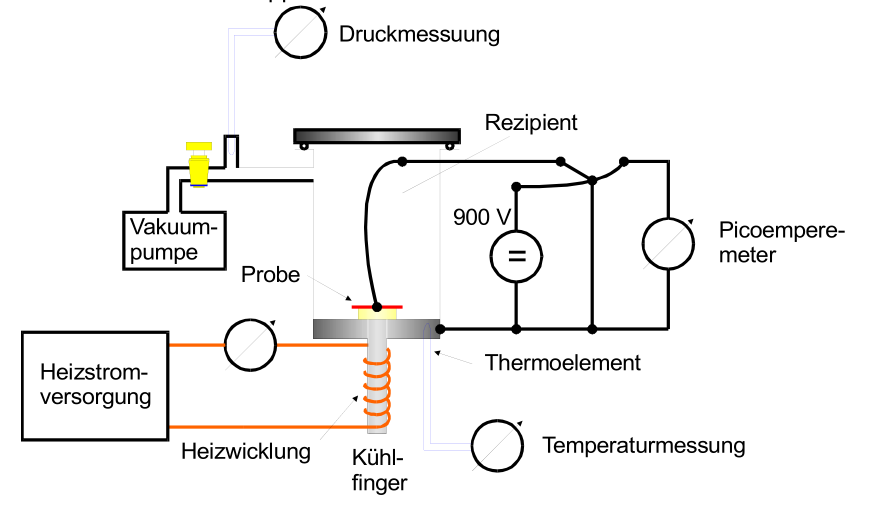
\includegraphics[width=0.7\textwidth]{aufbau.PNG}
    \caption{Aufbau der verwendeten Apparatur.\cite{skript}}
    \label{fig:aufbau}
\end{figure}\\
Zu Beginn wird der Kondensator mit $900\ \si{\volt}$ aufgeladen und die Probe auf $320\mathrm{K}$ erhitzt.
Beim Aufladen ist zu beachten, dass die Aufladezeit groß gegen die Relaxationszeit ist.
Anschließend wird die Probe, durch Eintauchen des Kühlfingers in Stickstoff,
auf $210\mathrm{K}$ gekühlt.
Das elektrische Feld wird nun abgestellt und der Kondensator zum Entladen kurzgeschlossen.
Zur Messung des Polarisationsstroms wird die Probe erneut auf $320\mathrm{K}$ erhitzt.
Beim Erhitzen werden in Abständen von einer Minute Strom-Temperatur-Paare mit dem Picoamperemeter aufgenommen.
Dieser Vorgang wird für zwei unterschiedliche Heizraten wiederholt.
